% =============================================================================
% APENDICE E: TABLAS Y FIGURAS COMPLEMENTARIAS
% (E.1-E.3 antiguas movidas en julio 2026: variables -> apendice A,
%  caracteristicas -> apendice B, ejemplos de estrategia -> apendice D)
% =============================================================================

\section{Tablas y Figuras Complementarias}
\label{sec:appendix_supplementary}

Este ap\'endice re\'une las tablas de soporte y figuras complementarias referenciadas en el cuerpo del trabajo, organizadas seg\'un la secci\'on a la que complementan.

% ---------------------------------------------------------------------------
% Revisi\'on de Literatura
% ---------------------------------------------------------------------------

\subsection{Figuras Complementarias de la Revisi\'on de Literatura}
\label{sec:appendix_lit_figures}

\begin{figure}[H]
\centering
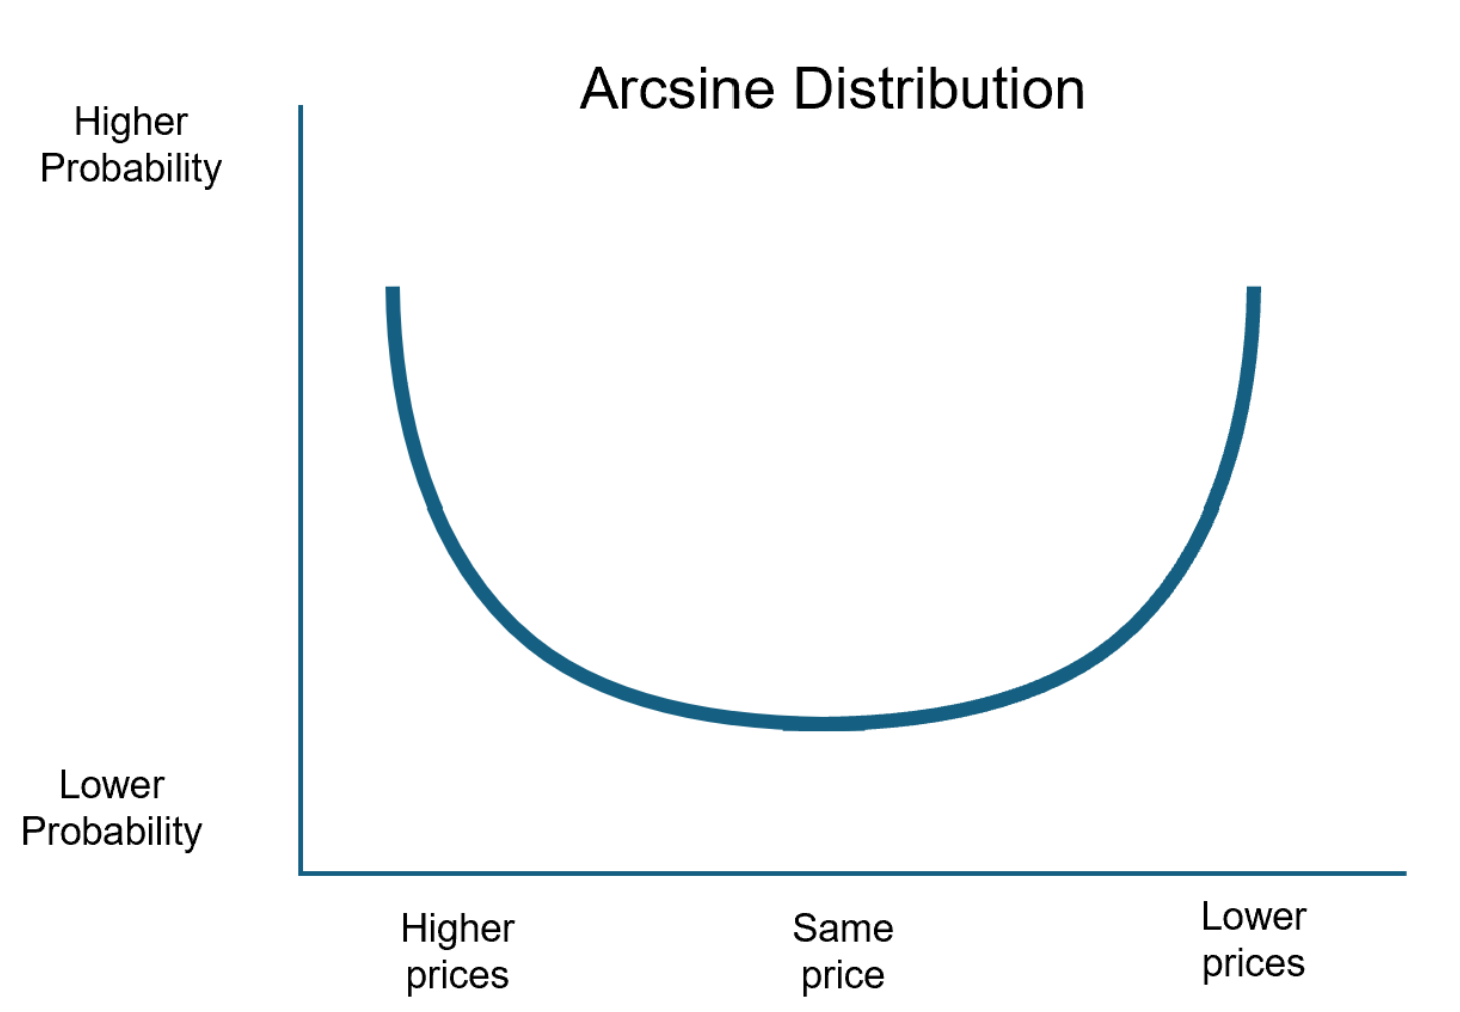
\includegraphics[width=0.75\textwidth]{figures/Law.png}
\caption{Distribuci\'on del arcoseno, donde la probabilidad de que un camino aleatorio permanezca en territorio de precios altos o bajos es mucho mayor que la de oscilar sim\'etricamente alrededor del precio inicial, generando tendencias persistentes de manera natural. Adaptado de \citet{cmt2020}.}
\label{fig:arcsine}
\end{figure}

% ---------------------------------------------------------------------------
% Resultados Emp\'iricos
% ---------------------------------------------------------------------------

\subsection{Tablas y Figuras de Resultados Emp\'iricos}
\label{sec:appendix_results_tables}

\begin{table}[htbp]
\centering
\caption{Distribuci\'on de Posiciones por Modelo (Estrategia Long-Only)}
\label{tab:position_distribution}
\small
\begin{tabular}{@{}lrrrrr@{}}
\toprule
\textbf{Modelo} & \textbf{UPRO (3x)} & \textbf{SPY (1x)} & \textbf{Cash (0)} & \textbf{Total Long} & \textbf{N\textdegree{} Trades} \\
\midrule
LSTM\_Attention & 12.2\% & 32.7\% & 55.1\% & 44.9\% & 465 \\
Ridge & 20.8\% & 17.0\% & 62.3\% & 37.7\% & 409 \\
RandomForest & 5.2\% & 16.9\% & 77.9\% & 22.1\% & 175 \\
CNN\_LSTM & 12.1\% & 28.6\% & 59.3\% & 40.7\% & 633 \\
DLinear & 6.6\% & 52.2\% & 41.2\% & 58.8\% & 788 \\
GradientBoosting & 4.2\% & 4.0\% & 91.9\% & 8.1\% & 11 \\
CatBoost & 4.0\% & 9.1\% & 86.9\% & 13.1\% & 224 \\
Theta & 2.3\% & 2.2\% & 95.5\% & 4.5\% & 36 \\
SeasonalNaive & 20.2\% & 39.7\% & 40.0\% & 60.0\% & 1042 \\
NBEATS & 13.9\% & 10.3\% & 75.8\% & 24.2\% & 507 \\
Lasso & 1.4\% & 4.8\% & 93.9\% & 6.1\% & 90 \\
GARCH & 1.7\% & 6.2\% & 92.1\% & 7.9\% & 126 \\
LightGBM & 3.7\% & 6.3\% & 90.0\% & 10.0\% & 134 \\
NHiTS & 7.1\% & 52.4\% & 40.4\% & 59.6\% & 805 \\
AutoARIMA & 0.0\% & 0.0\% & 100.0\% & 0.0\% & 0 \\
TCN & 7.7\% & 20.7\% & 71.6\% & 28.4\% & 383 \\
TFT & 21.4\% & 38.7\% & 39.9\% & 60.1\% & 804 \\
XGBoost & 29.1\% & 3.8\% & 67.1\% & 32.9\% & 42 \\
ElasticNet & 3.7\% & 9.4\% & 86.9\% & 13.1\% & 175 \\
Prophet & 2.3\% & 8.8\% & 88.9\% & 11.1\% & 77 \\
BiLSTM & 12.1\% & 20.1\% & 67.8\% & 32.2\% & 546 \\
ExponentialSmoothing & 26.7\% & 45.3\% & 28.0\% & 72.0\% & 904 \\
BiGRU & 15.7\% & 27.5\% & 56.8\% & 43.2\% & 752 \\
\bottomrule
\end{tabular}
\begin{tablenotes}
\small
\item Nota: Porcentajes representan la proporci\'on de d\'ias en cada posici\'on. UPRO = 3x apalancado largo, SPY = 1x largo, Cash = tasa libre de riesgo. N\'umero de trades = cambios de posici\'on.
\end{tablenotes}
\end{table}


\begin{table}[H]
\centering
\caption{Estad\'isticas de Trading por Modelo (Top 5)}
\label{tab:trading_stats}
\small
\begin{tabular}{@{}lrrrrr@{}}
\toprule
\textbf{Modelo} & \textbf{N Trades} & \textbf{Win Rate} & \textbf{Avg Win} & \textbf{Avg Loss} & \textbf{Profit Factor} \\
\midrule
LSTM+Attention & 465 & 53.9\% & +1.5\% & $-$1.2\% & 1.52 \\
Ridge & 409 & 55.8\% & +1.9\% & $-$1.8\% & 1.35 \\
RandomForest & 175 & 52.8\% & +1.6\% & $-$1.2\% & 1.49 \\
CNN-LSTM & 633 & 51.4\% & +1.4\% & $-$1.1\% & 1.29 \\
DLinear & 788 & 53.6\% & +0.9\% & $-$0.9\% & 1.16 \\
\bottomrule
\end{tabular}
\vspace{0.2cm}
\parbox{0.9\textwidth}{\footnotesize\textit{Nota: N Trades = cambios de posici\'on. Win Rate, Avg Win, Avg Loss y Profit Factor calculados sobre d\'ias activos (posici\'on $\neq$ 0). Profit Factor = $|$Avg Win / Avg Loss$|$.}}
\end{table}

\begin{table}[H]
\centering
\caption{Modelos Ganadores vs M\'ultiples Benchmarks}
\label{tab:benchmarks}
\begin{tabular}{@{}lrrrr@{}}
\toprule
\textbf{Estrategia} & \textbf{Ret. Total} & \textbf{Sharpe} & \textbf{Max DD} & \textbf{Calmar} \\
\midrule
LSTM+Attention & +395\% & 1.32 & $-$20.5\% & 1.77 \\
Ridge & +253\% & 0.86 & $-$31.8\% & 0.87 \\
RandomForest & +128\% & 0.65 & $-$15.0\% & 1.15 \\
CNN-LSTM & +122\% & 0.57 & $-$35.9\% & 0.47 \\
\midrule
SPY Buy \& Hold & +101.3\% & 0.66 & $-$25.4\% & 0.57 \\
UPRO 3x (B\&H) & +122.8\% & 0.26 & $-$69.0\% & 0.24 \\
60/40 Portfolio & +70.6\% & 0.67 & $-$21.1\% & 0.52 \\
\bottomrule
\end{tabular}
\vspace{0.2cm}
\parbox{0.9\textwidth}{\footnotesize\textit{Nota: UPRO 3x B\&H incluye \textit{expense ratio} (0.91\%/a\~no) y \textit{bid-ask spread}; el \textit{volatility decay} est\'a impl\'icito en la composici\'on diaria de retornos 3$\times$. 60/40 = 60\% SPY + 40\% LF98TRUU Index (Bloomberg US Aggregate Bond Total Return) con rebalanceo mensual.}}
\end{table}

\begin{figure}[H]
\centering
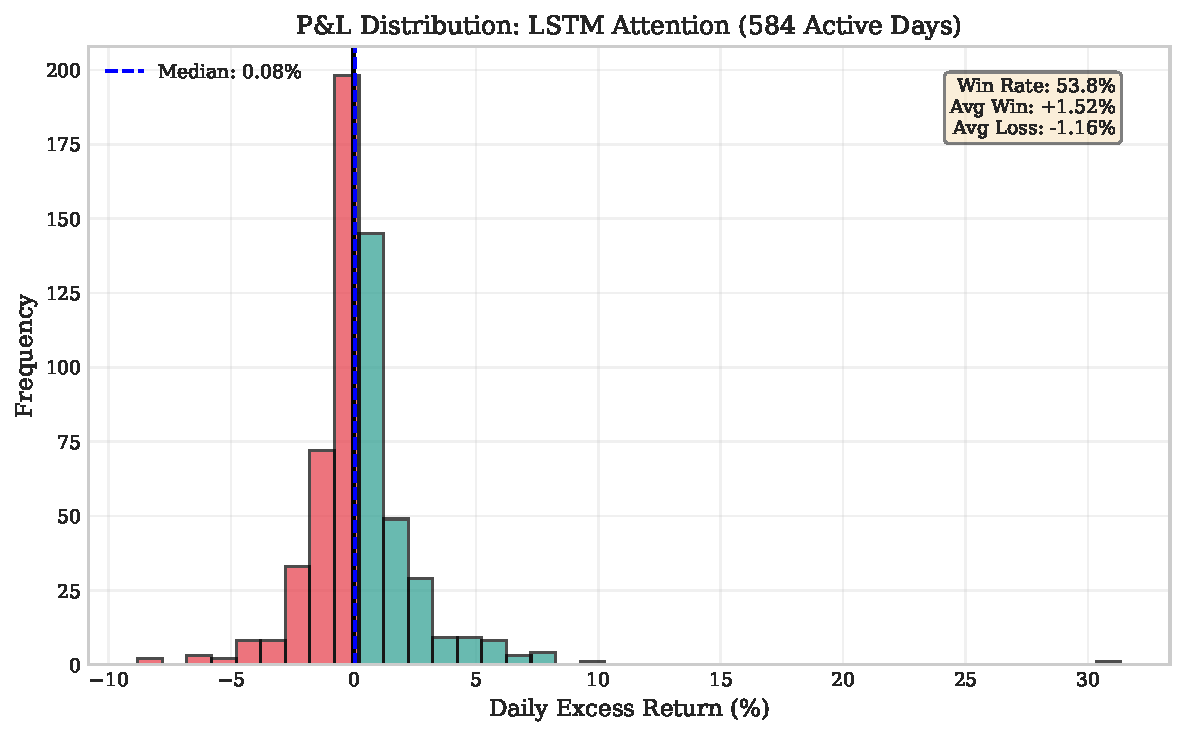
\includegraphics[width=0.8\textwidth]{figures/pnl_distribution_lstm_attention.pdf}
\caption{Distribuci\'on de retornos diarios en exceso sobre la tasa libre de riesgo del modelo LSTM+Attention. Histograma calculado sobre los d\'ias activos (posici\'on $\neq$ 0). Verde = d\'ias ganadores, Rojo = d\'ias perdedores. L\'inea vertical en 0\%.}
\label{fig:pnl_distribution}
\end{figure}

% ---------------------------------------------------------------------------
% Gesti\'on de Riesgo
% ---------------------------------------------------------------------------

\subsection{Tablas de Gesti\'on de Riesgo}
\label{sec:appendix_risk_tables}

\begin{table}[H]
\centering
\caption{Value at Risk y Expected Shortfall al 95\% por horizonte temporal}
\label{tab:var_cvar}
\small
\begin{tabular}{@{}lrrrr@{}}
\toprule
\textbf{Modelo} & \textbf{VaR 95\% (30d)} & \textbf{CVaR 95\% (30d)} & \textbf{VaR 95\% (90d)} & \textbf{CVaR 95\% (90d)} \\
\midrule
LSTM+Attention & $-6.18\%$ & $-10.39\%$ & $-3.77\%$ & $-6.51\%$ \\
Ridge & $-11.25\%$ & $-19.71\%$ & $-14.33\%$ & $-21.88\%$ \\
RandomForest & $-3.87\%$ & $-5.75\%$ & $-0.67\%$ & $-3.18\%$ \\
CNN-LSTM & $-9.02\%$ & $-14.84\%$ & $-16.29\%$ & $-23.05\%$ \\
\midrule
SPY (B\&H) & $-7.81\%$ & $-10.83\%$ & $-10.80\%$ & $-13.85\%$ \\
\bottomrule
\end{tabular}
\vspace{0.2cm}
\parbox{0.9\textwidth}{\footnotesize\textit{Nota: VaR y CVaR calculados sobre retornos acumulados en ventanas m\'oviles de 30 y 90 d\'ias de operaci\'on (1,272 y 1,212 ventanas respectivamente).}}
\end{table}

\begin{table}[H]
\centering
\caption{An\'alisis de m\'aximo \textit{drawdown} por modelo}
\label{tab:drawdown_detail}
\small
\begin{tabular}{@{}lrllrr@{}}
\toprule
\textbf{Modelo} & \textbf{MaxDD} & \textbf{Pico} & \textbf{Valle} & \textbf{Duraci\'on} & \textbf{Recuperaci\'on} \\
\midrule
LSTM+Attention & $-20.5\%$ & 2025-02-18 & 2025-04-07 & 34 d\'ias & 1 d\'ia \\
Ridge & $-31.8\%$ & 2021-09-14 & 2022-03-07 & 120 d\'ias & 56 d\'ias \\
RandomForest & $-15.0\%$ & 2022-04-01 & 2022-05-19 & 33 d\'ias & 23 d\'ias \\
CNN-LSTM & $-35.9\%$ & 2022-03-24 & 2022-07-15 & 77 d\'ias & 566 d\'ias \\
\midrule
SPY (B\&H) & $-25.4\%$ & 2021-12-31 & 2022-10-11 & 195 d\'ias & 318 d\'ias \\
\bottomrule
\end{tabular}
\vspace{0.2cm}
\parbox{0.9\textwidth}{\footnotesize\textit{Nota: Duraci\'on = d\'ias de operaci\'on desde el pico hasta el valle. Recuperaci\'on = d\'ias desde el valle hasta alcanzar un nuevo m\'aximo.}}
\end{table}

% ---------------------------------------------------------------------------
% Validaci\'on Estad\'istica
% ---------------------------------------------------------------------------

\subsection{Tablas de Validaci\'on Estad\'istica}
\label{sec:appendix_validation_tables}

\begin{table}[H]
\centering
\caption{Intervalos de confianza del Sharpe Ratio (\textit{bootstrap} 95\%, $B = 5{,}000$)}
\label{tab:sharpe_ci}
\small
\begin{tabular}{@{}lrrrrr@{}}
\toprule
\textbf{Modelo} & \textbf{Sharpe} & \textbf{IC 95\% Inf} & \textbf{IC 95\% Sup} & \textbf{P(S$>$0)} & \textbf{P(S$>$SPY)} \\
\midrule
LSTM+Attention & 1.319 & 0.375 & 2.424 & 99.6\% & 83.1\% \\
Ridge & 0.856 & $-$0.121 & 2.115 & 94.9\% & 60.4\% \\
RandomForest & 0.651 & $-$0.218 & 1.480 & 93.3\% & 49.9\% \\
CNN-LSTM & 0.572 & $-$0.292 & 1.485 & 89.3\% & 44.4\% \\
\midrule
SPY (B\&H) & 0.657 & $-$0.253 & 1.730 & 91.4\% & -- \\
\bottomrule
\end{tabular}
\vspace{0.2cm}
\parbox{0.9\textwidth}{\footnotesize\textit{Nota: P(S$>$0) = probabilidad de Sharpe positivo. P(S$>$SPY) = probabilidad de superar el Sharpe del benchmark. Intervalos calculados con 5{,}000 iteraciones bootstrap, semilla 42.}}
\end{table}

\begin{table}[H]
\centering
\caption{Test de Diebold-Mariano (retornos de estrategia vs SPY \textit{Buy \& Hold})}
\label{tab:dm_test}
\small
\begin{tabular}{@{}lrrr@{}}
\toprule
\textbf{Modelo} & \textbf{Estad\'istico DM} & \textbf{p-valor (1 cola)} & \textbf{Significativo (5\%)} \\
\midrule
LSTM+Attention & 2.296 & 0.0108 & S\'i \\
Ridge & 1.275 & 0.1012 & No \\
RandomForest & 0.363 & 0.3584 & No \\
CNN-LSTM & 0.325 & 0.3725 & No \\
\bottomrule
\end{tabular}
\vspace{0.2cm}
\parbox{0.9\textwidth}{\footnotesize\textit{Nota: $DM > 0$ indica que la estrategia genera retornos superiores al \textit{benchmark}. Correcci\'on Newey-West con 5 rezagos. Hip\'otesis alternativa unidireccional (estrategia $>$ \textit{benchmark}).}}
\end{table}

\begin{table}[H]
\centering
\caption{Test de Clark-West (predicciones vs media hist\'orica del entrenamiento)}
\label{tab:cw_test}
\small
\begin{tabular}{@{}lrrr@{}}
\toprule
\textbf{Modelo} & \textbf{CW Stat} & \textbf{p-valor (1 cola)} & \textbf{Conclusi\'on} \\
\midrule
LSTM+Attention & 1.901 & 0.029 & Rechaza $H_0$ (5\%) \\
Ridge & 1.215 & 0.112 & No rechaza \\
CNN-LSTM & 0.641 & 0.261 & No rechaza \\
RandomForest & $-$0.336 & 0.631 & No rechaza \\
\bottomrule
\end{tabular}
\vspace{0.2cm}
\parbox{0.9\textwidth}{\footnotesize\textit{Nota: $H_0$ establece que el modelo no posee capacidad predictiva superior a la media hist\'orica. Test de una cola. Correcci\'on Newey-West con 5 rezagos.}}
\end{table}

\begin{table}[H]
\centering
\caption{Degradaci\'on de m\'etricas predictivas entre entrenamiento y prueba}
\label{tab:overfitting}
\small
\begin{tabular}{@{}lrrrr@{}}
\toprule
\textbf{Modelo} & \textbf{DA Train} & \textbf{DA Test} & \textbf{Degradaci\'on DA} & \textbf{MSE Test/Train} \\
\midrule
LSTM+Attention & 0.492 & 0.470 & $-$4.6\% & 0.68$\times$ \\
CNN-LSTM & 0.501 & 0.455 & $-$9.3\% & 0.87$\times$ \\
Ridge & 0.575 & 0.468 & $-$18.6\% & 2.55$\times$ \\
RandomForest & 0.580 & 0.459 & $-$20.9\% & 1.86$\times$ \\
\midrule
XGBoost & 0.552 & 0.543 & $-$1.6\% & 0.89$\times$ \\
\bottomrule
\end{tabular}
\vspace{0.2cm}
\parbox{0.9\textwidth}{\footnotesize\textit{Nota: DA = \textit{directional accuracy} (proporci\'on de predicciones con signo correcto). MSE Test/Train $> 1$ indica que el error cuadr\'atico medio aumenta en el per\'iodo fuera de muestra. XGBoost se incluye como ejemplo de modelo degenerado (Sharpe test = $-$0.024).}}
\end{table}

% ---------------------------------------------------------------------------
% Costos de Transacci\'on
% ---------------------------------------------------------------------------

\subsection{Tablas y Figuras de Costos de Transacci\'on}
\label{sec:appendix_cost_tables}

\begin{table}[H]
\centering
\caption{Par\'ametros de Costo por Instrumento}
\label{tab:tx_costs_detail}
\begin{tabular}{@{}lrrr@{}}
\toprule
\textbf{Instrumento} & \textbf{Bid-Ask} & \textbf{Expense Ratio} & \textbf{Round-Trip} \\
\midrule
UPRO (3x Long) & 5 bps & 0.91\%/a\~no & 10 bps \\
SPY (1x Long) & 2 bps & 0.09\%/a\~no & 4 bps \\
Cash & 0 bps & 0\% & 0 bps \\
\bottomrule
\end{tabular}
\vspace{0.2cm}
\parbox{0.9\textwidth}{\footnotesize\textit{Nota: Round-trip = bid-ask de entrada + bid-ask de salida. Expense ratio aplicado diariamente como ratio anual / 252.}}
\end{table}

\begin{table}[H]
\centering
\caption{Impacto de Costos de Transacci\'on por Modelo}
\label{tab:cost_breakdown}
\small
\begin{tabular}{@{}lrrrrr@{}}
\toprule
\textbf{Modelo} & \textbf{Capital Final} & \textbf{P\&L Bruto} & \textbf{Tx Costs} & \textbf{Tx/P\&L} & \textbf{Trades} \\
\midrule
LSTM\_Attention & \$49,538 & \textcolor{ForestGreen}{\$52,996} & \$13,459 & 25.4\% & 465 \\
Ridge & \$35,254 & \textcolor{ForestGreen}{\$36,983} & \$11,729 & 31.7\% & 409 \\
RandomForest & \$22,749 & \textcolor{ForestGreen}{\$15,148} & \$2,398 & 15.8\% & 175 \\
CNN\_LSTM & \$22,222 & \textcolor{ForestGreen}{\$20,022} & \$7,800 & 39.0\% & 633 \\
DLinear & \$16,771 & \textcolor{ForestGreen}{\$11,584} & \$4,813 & 41.5\% & 788 \\
GradientBoosting & \$16,629 & \textcolor{ForestGreen}{\$7,061} & \$432 & 6.1\% & 11 \\
CatBoost & \$14,601 & \textcolor{ForestGreen}{\$6,169} & \$1,568 & 25.4\% & 224 \\
Theta & \$14,442 & \textcolor{ForestGreen}{\$4,954} & \$512 & 10.3\% & 36 \\
NBEATS & \$14,387 & \textcolor{ForestGreen}{\$8,824} & \$4,437 & 50.3\% & 507 \\
\rowcolor{naivebg} SeasonalNaive$^\dagger$ & \$14,300 & \textcolor{ForestGreen}{\$12,816} & \$8,516 & 66.4\% & 1042 \\
Lasso & \$13,768 & \textcolor{ForestGreen}{\$4,379} & \$611 & 13.9\% & 90 \\
GARCH & \$12,659 & \textcolor{ForestGreen}{\$3,337} & \$679 & 20.3\% & 126 \\
LightGBM & \$12,553 & \textcolor{ForestGreen}{\$3,588} & \$1,035 & 28.8\% & 134 \\
NHiTS & \$12,141 & \textcolor{ForestGreen}{\$6,043} & \$3,902 & 64.6\% & 805 \\
AutoARIMA & \$11,827 & \textcolor{ForestGreen}{\$1,827} & \$0 & 0.0\% & 0 \\
TCN & \$11,796 & \textcolor{ForestGreen}{\$3,876} & \$2,080 & 53.7\% & 383 \\
TFT & \$11,350 & \textcolor{ForestGreen}{\$7,571} & \$6,221 & 82.2\% & 804 \\
Prophet & \$10,784 & \textcolor{ForestGreen}{\$1,221} & \$436 & 35.7\% & 77 \\
ElasticNet & \$10,779 & \textcolor{ForestGreen}{\$1,894} & \$1,116 & 58.9\% & 175 \\
XGBoost & \$10,710 & \textcolor{ForestGreen}{\$3,167} & \$2,457 & 77.6\% & 42 \\
BiLSTM & \$10,494 & \textcolor{ForestGreen}{\$3,625} & \$3,131 & 86.4\% & 546 \\
ExponentialSmoothing & \$8,463 & \textcolor{ForestGreen}{\$4,473} & \$6,011 & 134.4\% & 904 \\
BiGRU & \$6,683 & \textcolor{BrickRed}{\$-436} & \$2,881 & -- & 752 \\
\midrule
\textit{Promedio} & -- & -- & \$3,749 & -- & 397 \\
\bottomrule
\end{tabular}
\begin{tablenotes}
\small
\item Nota: Capital inicial = \$10,000. \colorbox{naivebg}{$^\dagger$SeasonalNaive} = \textit{benchmark} de complejidad m\'inima. Tx Costs incluye bid-ask spreads (UPRO 5 bps, SPY 2 bps por operaci\'on; 10 y 4 bps ida y vuelta), expense ratios y volatility drag. Tx/P\&L = proporci\'on de costos respecto a ganancias brutas.
\end{tablenotes}
\end{table}


\begin{table}[H]
\centering
\caption{Validaci\'on de Par\'ametros de Costo, Estudio vs.\ Mercado Real}
\label{tab:cost_validation}
\small
\begin{tabular}{@{}llllr@{}}
\toprule
\textbf{Par\'ametro} & \textbf{Este estudio} & \textbf{Mercado real} & \textbf{Fuente} & \textbf{Ratio} \\
\midrule
Expense ratio UPRO & 0.91\%/a\~no & 0.89\%/a\~no & ProShares\textsuperscript{a} & 1.02$\times$ \\
Expense ratio SPY & 0.09\%/a\~no & 0.0945\%/a\~no & State Street\textsuperscript{b} & 0.95$\times$ \\
Bid-ask UPRO & 5 bps & 2 bps & ProShares\textsuperscript{a} (mediana 30d) & 2.50$\times$ \\
Bid-ask SPY & 2 bps & $\approx$0 bps & State Street\textsuperscript{b} (mediana 30d) & $>$2.5$\times$ \\
$\sigma$ diaria (vol drag) & realizada 21d & 0.95--1.26\% & S\&P 500 hist\'orico & $\sim$1.0$\times$ \\
\bottomrule
\end{tabular}
\vspace{0.2cm}
\parbox{0.9\textwidth}{\footnotesize\textit{Nota: \textsuperscript{a}ProShares reporta un expense ratio de 0.89\% bajo un fee waiver contractual vigente hasta septiembre 2026. \textsuperscript{b}State Street reporta un gross expense ratio de 0.0945\% y una mediana de bid-ask spread de 0.00\% a 30 d\'ias. Datos consultados en julio 2026 desde las p\'aginas oficiales de los emisores.}}
\end{table}

\begin{table}[H]
\centering
\caption{Sensibilidad del Retorno a Costos de Transacci\'on}
\label{tab:cost_sensitivity}
\small
\begin{tabular}{@{}lrrrrr@{}}
\toprule
\textbf{Modelo} & \textbf{Ret.\ Base} & \textbf{+50\% Costos} & \textbf{+100\% Costos} & \textbf{Break-even} & \textbf{Tx/P\&L} \\
\midrule
LSTM+Attention & +395\% & +328\% & +261\% & 3.9$\times$ & 25.4\% \\
Ridge & +253\% & +194\% & +135\% & 3.2$\times$ & 31.7\% \\
RandomForest & +128\% & +116\% & +103\% & 6.3$\times$ & 15.8\% \\
CNN-LSTM & +122\% & +83\% & +44\% & 2.6$\times$ & 39.0\% \\
\bottomrule
\end{tabular}
\vspace{0.2cm}
\parbox{0.9\textwidth}{\footnotesize\textit{Nota: Aproximaci\'on lineal donde el retorno ajustado $\approx$ (P\&L bruto $-$ costos $\times$ multiplicador) / capital inicial. Break-even = P\&L bruto / costos totales, es decir, el multiplicador m\'aximo de costos antes de que la estrategia genere p\'erdidas. Tx/P\&L = costos totales como porcentaje del P\&L bruto.}}
\end{table}

\begin{figure}[H]
\centering
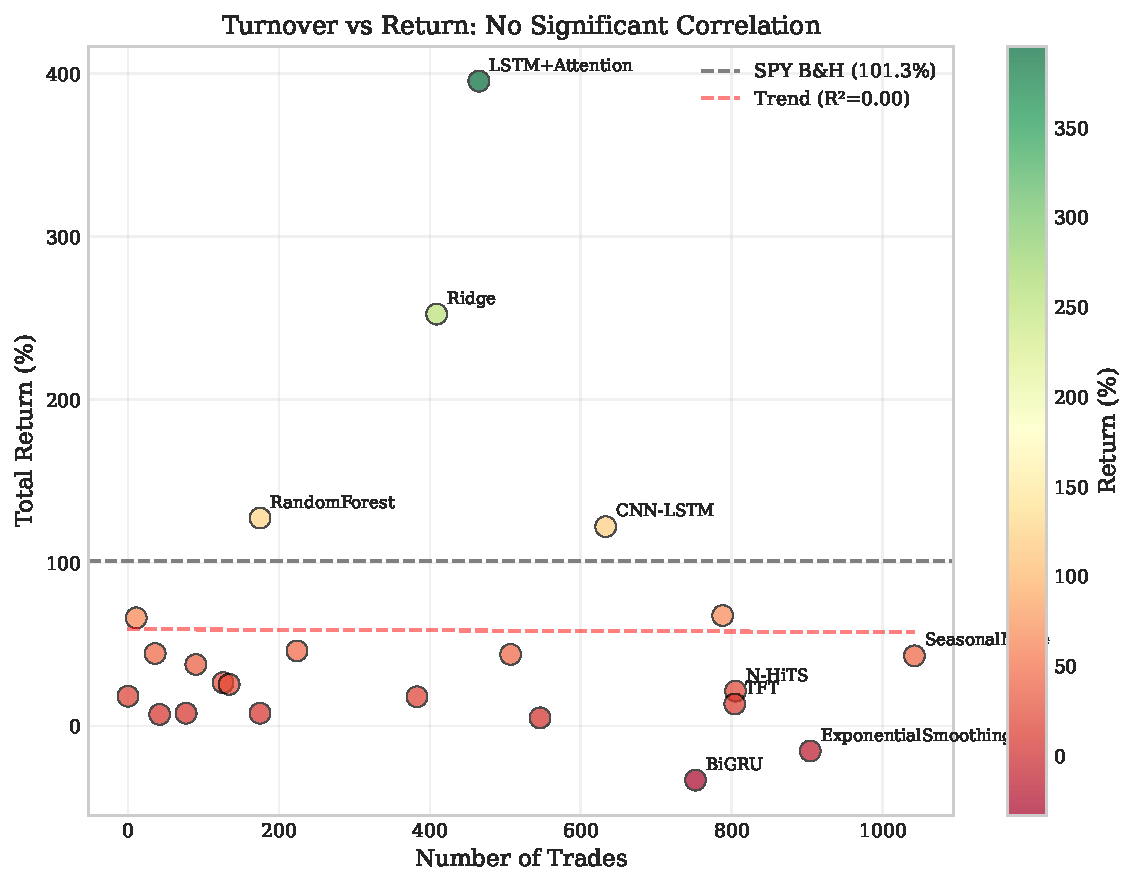
\includegraphics[width=0.8\textwidth]{figures/turnover_vs_return.pdf}
\caption{Relaci\'on entre \textit{turnover} (n\'umero de \textit{trades}) y retorno neto. Cada punto representa un modelo. La l\'inea punteada representa la regresi\'on lineal ($R^2 = 0.00$).}
\label{fig:turnover_return}
\end{figure}
